\documentclass{beamer}
\usetheme{Madrid}
\usepackage{listings}
\usepackage{xcolor}

% Define SUSE green color
\definecolor{susegreen}{RGB}{48,186,120}
\setbeamercolor{structure}{fg=susegreen}
\setbeamercolor{palette primary}{bg=susegreen,fg=white}
\setbeamercolor{palette secondary}{bg=susegreen!80,fg=white}
\setbeamercolor{palette tertiary}{bg=susegreen!60,fg=white}
\setbeamercolor{palette quaternary}{bg=susegreen!40,fg=black}

\lstset{
    basicstyle=\ttfamily\tiny,
    breaklines=true,
    frame=single,
    language=Python,
    showstringspaces=false
}

\title{Song Search using CLAP}
\subtitle{SUSE Hack Week 25}
\date{}

\begin{document}

% Title Slide
\begin{frame}
\titlepage
\vspace{-0.5cm}
\begin{center}
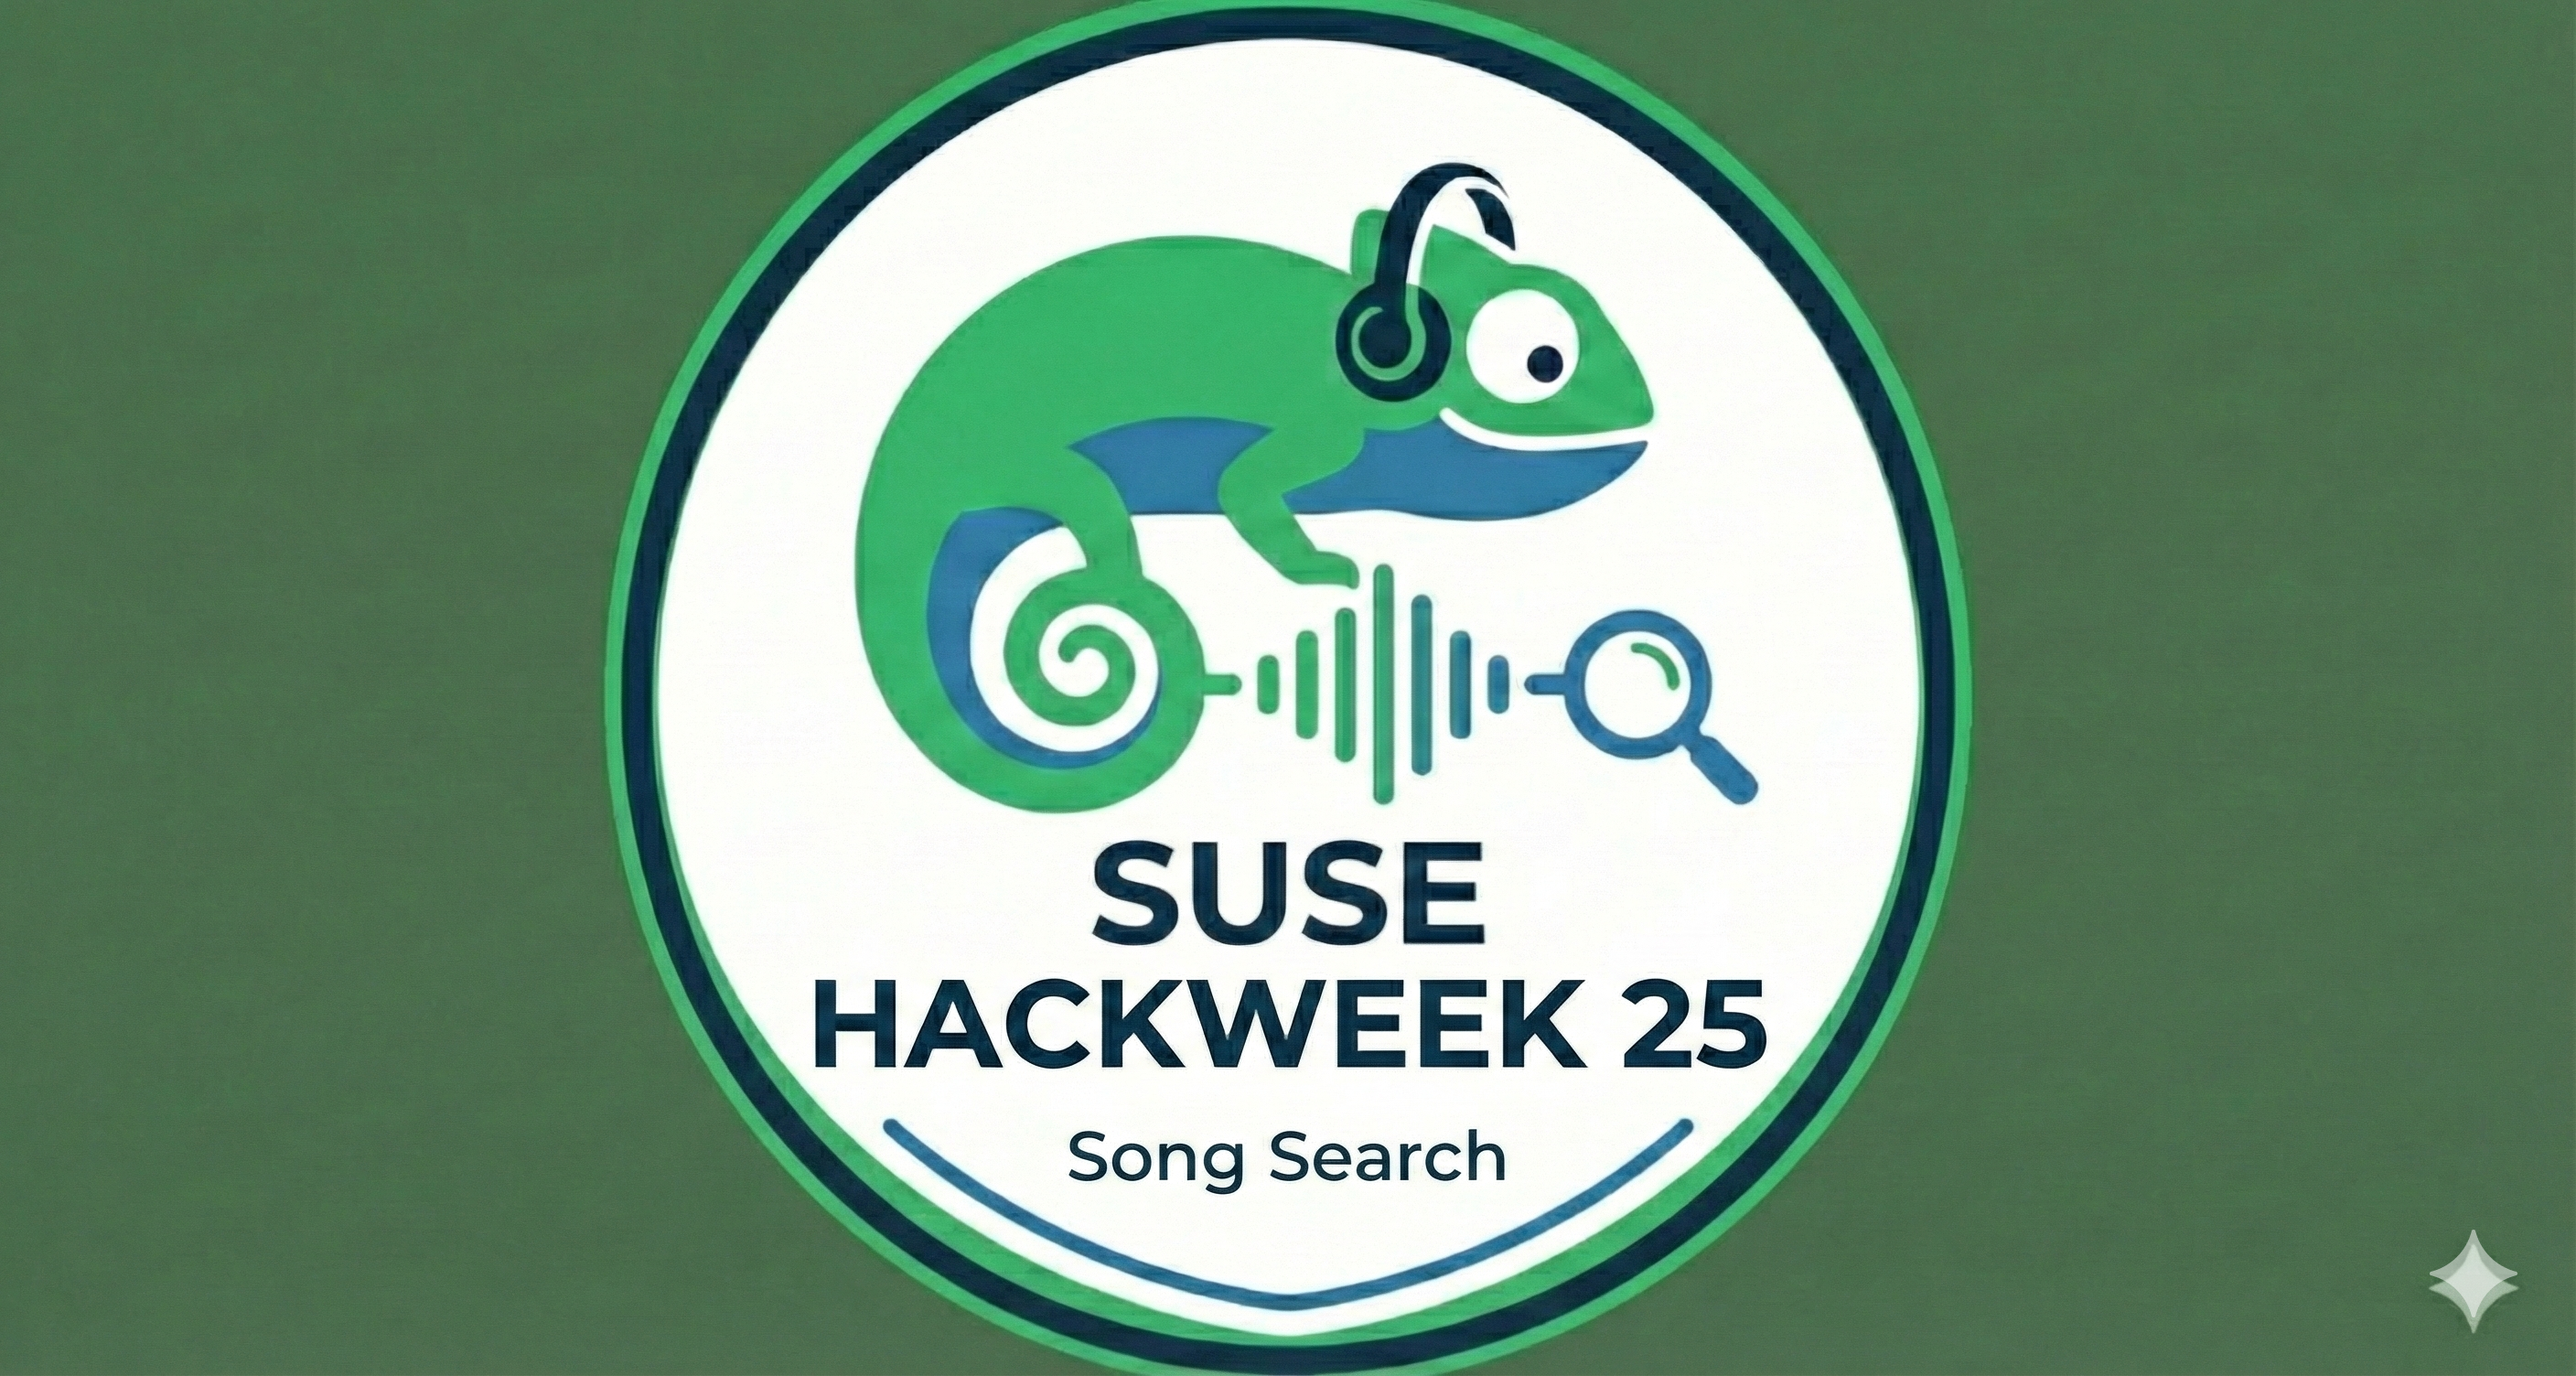
\includegraphics[width=0.7\textwidth]{../HW25-SONG-SEARCH.png}
\end{center}
\end{frame}

% Slide 2: Goals
\begin{frame}{Goals}
\textbf{Search music using natural language descriptions}

\vspace{0.6cm}

\begin{itemize}
    \item Find songs by describing what you hear: "piano melody", "female vocalist"
    \item Compare songs to find similar tracks
    \item Experiment AI with Copilot Code Assistant
\end{itemize}
\end{frame}

% Slide 3: CLAP Overview
\begin{frame}{CLAP Overview}
\textbf{CLAP} (Contrastive Language-Audio Pretraining) - Bridging audio and language

\vspace{0.4cm}

\textbf{Core Concept:}

CLAP can represent both songs and text descriptions as \textbf{512-dimensional vectors} in the same mathematical space. This enables searching for music using natural language queries.

\vspace{0.3cm}

\textbf{How it works:}
\begin{itemize}
    \item A song becomes a 512-number vector capturing its audio characteristics
    \item A text query like "piano music" also becomes a 512-number vector
    \item Vectors that point in similar directions represent similar content
    \item We measure similarity to find songs matching the description
\end{itemize}

\vspace{0.3cm}

\textbf{Model:} \texttt{music\_audioset\_epoch\_15\_esc\_90.14.pt} - Specialized for music (71\% genre accuracy, trained on \textasciitilde{}4M samples)
\end{frame}

% Slide 4: Implementation
\begin{frame}{Implementation}
\textbf{Two Modes:}

\begin{itemize}
    \item \textbf{Single Analysis:} \texttt{single\_analysis.py} - One song vs one query
    \item \textbf{Batch Analysis:} \texttt{multiple\_analysis.py} - All songs vs all queries
\end{itemize}

\vspace{0.3cm}

\textbf{Architecture:}
\begin{itemize}
    \item \texttt{clap\_analysis.py} - Core library (shared)
    \item Automatic model download \& caching
    \item Parallel processing across CPU cores
    \item CSV output with detailed metrics
\end{itemize}

\vspace{0.3cm}

\textbf{Cosine Similarity Scores:}
\begin{itemize}
    \item Range: $-1$ (opposite) to $+1$ (identical)
    \item Thresholds: $> 0.3$ = HIGH, $> 0.15$ = MODERATE, $\leq 0.15$ = LOW
\end{itemize}
\end{frame}

% Slide 5: Output Example - Classical
\begin{frame}{Output Example - Classical}
\textbf{Song:} Aaron Dunn - Minuet (Classical Piano)

\vspace{0.2cm}

\begin{table}[h]
\tiny
\begin{tabular}{p{3.2cm}|p{3.2cm}|p{3.2cm}}
\textbf{HIGH ($> 0.3$)} & \textbf{MODERATE ($> 0.15$)} & \textbf{LOW ($\leq 0.15$)} \\
\hline
\textbf{0.41} piano & \textbf{0.29} chill & \textbf{0.15} 70s \\
\textbf{0.40} \textcolor{susegreen}{classical instrumental song with piano} & \textbf{0.28} chillout & \textbf{0.14} choir \\
\textbf{0.38} classical music & \textbf{0.27} sad & \textbf{0.14} beautiful \\
\textbf{0.37} instrumental & \textbf{0.26} jazz & \textbf{0.14} danceable \\
\textbf{0.33} instrumental music & \textbf{0.25} acoustic & \textbf{0.12} pop music wit bass guitar \\
\textbf{} & \textbf{0.23} acoustic guitar & \textbf{0.12} funk \\
\textbf{} & \textbf{0.22} pop & \textbf{0.12} bass guitar \\
\textbf{} & \textbf{0.21} folk & \textbf{0.11} soul \\
\textbf{} & \textbf{0.21} happy & \textbf{0.11} rock \\
\end{tabular}
\end{table}

\vspace{0.2cm}

\small
\textbf{Observation:} Piano and classical-related queries score highest. Chill/mellow descriptors moderate. Rock and modern era queries score low.

\vspace{0.2cm}

\textbf{Tip:} \textcolor{susegreen}{Detailed, specific queries} combining multiple descriptors (genre + instrument + style) yield excellent results!
\end{frame}

% Slide 6: Output Example - Rock
\begin{frame}{Output Example - Rock}
\textbf{Song:} SUSE Band - Paint it Green (Rock)

\vspace{0.2cm}

\begin{table}[h]
\tiny
\begin{tabular}{p{3.2cm}|p{3.2cm}|p{3.2cm}}
\textbf{HIGH ($> 0.3$)} & \textbf{MODERATE ($> 0.15$)} & \textbf{LOW ($\leq 0.15$)} \\
\hline
\textbf{0.42} indie rock & \textbf{0.28} hard rock & \textbf{0.14} heavy metal \\
\textbf{0.41} alternative rock & \textbf{0.28} folk & \textbf{0.14} dance \\
\textbf{0.40} classic rock & \textbf{0.26} punk & \textbf{0.13} soul \\
\textbf{0.37} Progressive rock & \textbf{0.25} 80s & \textbf{0.13} instrumental \\
\textbf{0.37} indie pop & \textbf{0.25} funk & \textbf{0.13} acoustic guitar \\
\textbf{0.36} rock & \textbf{0.25}90s & \textbf{0.13} singing \\
\textbf{0.33} \textcolor{red}{female vocalist} & \textbf{0.24}60s & \textbf{0.12} bass guitar \\
\textbf{0.32} rock music & \textbf{0.24} metal & \textbf{0.12} guitar \\
\textbf{0.31} blues & \textbf{0.23} Mellow & \textbf{0.06} \textcolor{red}{female voice} \\
\end{tabular}
\end{table}

\vspace{0.2cm}

\small
\textbf{Observation:} Rock subgenres (indie, alternative, classic) score highest. Generic instrument queries score low.

\vspace{0.2cm}

\textbf{Query Wording Matters:} Notice \textcolor{red}{"female vocalist"} (0.33, HIGH) vs \textcolor{red}{"female voice"} (0.06, LOW) - 5× difference! Use music industry vocabulary for better results.
\end{frame}

% Slide 7: Song-to-Song Similarity
\begin{frame}{Finding Similar Songs}
\textbf{Bonus Feature:} Beyond text search, we can find which songs sound similar to each other.

\vspace{0.3cm}

\textbf{Example:} Finding songs similar to SUSE Band - Paint it Green (Rock)

\begin{table}[h]
\small
\begin{tabular}{lc}
\textbf{Song} & \textbf{Similarity} \\
\hline
HoliznaCC0 - Dreams Of Lilith (Rock) & 0.72 \\
Jenna Jay - Someone Real (Pop) & 0.56 \\
Zane Little - Always and Forever (Pop) & 0.47 \\
SUSE Band - SUSE Yes Please (Pop) & 0.43 \\
SUSE Band - Can't Stop The SUSE (Pop) & 0.39 \\
Aaron Dunn - Minuet (Classical Piano) & 0.18 \\
\hline
\end{tabular}
\end{table}

\vspace{0.3cm}

\textbf{Use Cases:}
\begin{itemize}
    \item Find songs with similar instrumentation or mood
    \item Create automatic playlists based on audio similarity
    \item Discover patterns in your music collection
\end{itemize}
\end{frame}

% Slide 7: AI Support - What Went Well
\begin{frame}{AI Support in Development - What Went Well}
\textbf{Project developed with GitHub Copilot (Claude Sonnet 4.5)}

\textbf{1. Research \& Model Selection}
\begin{itemize}
    \item Compared CLAP models → selected \texttt{music\_audioset} (71\% GTZAN accuracy)
    \item Read CLAP paper, explained architecture accessibly
\end{itemize}

\textbf{2. Code Analysis \& Technical Discovery}
\begin{itemize}
    \item Examined checkpoint: model lacks fusion, max 10s segments
    \item Designed overlapping segment solution
\end{itemize}

\textbf{3. Data Analysis \& Documentation}
\begin{itemize}
    \item Found "vocalist" vs "voice" pattern (5x difference in results)
    \item Generated all technical docs with examples
\end{itemize}
\end{frame}

% Slide 8: AI Support - What Needs Improvement
\begin{frame}{AI Support in Development - What Needs Improvement}
\textbf{1. Unrequested Code Changes}
\begin{itemize}
    \item Single-file CLI disappeared, score icons changed without asking
    \item \textbf{Problem:} Full file rewrites hide unintended changes
    \item \textbf{Lesson:} Always review diffs carefully
\end{itemize}

\textbf{2. First Solution $\neq$ Best Solution}
\begin{itemize}
    \item \textbf{Performance:} Song analyzed per query → challenged → \textbf{15x faster}
    \item \textbf{Threading:} Single-threaded → asked "faster?" → multiprocessing
\end{itemize}

\textbf{Key Lesson:} Working $\neq$ optimal. Challenge AI with domain knowledge.
\end{frame}

% Slide 9: Best Practices for AI Collaboration
\begin{frame}{Best Practices for AI-Assisted Development}
\textbf{Do's:}
\begin{itemize}
    \item Ask AI to research and compare options (models, approaches)
    \item Request code analysis to understand existing implementations
    \item Share actual data/errors for pattern recognition
    \item Challenge solutions: "Can this be faster?" "Is there a better way?"
    \item Request documentation with examples from your project
\end{itemize}

\vspace{0.3cm}

\textbf{Don'ts:}
\begin{itemize}
    \item Don't accept first working solution as optimal
    \item Don't let AI rewrite entire files without showing diffs
    \item Don't assume AI made only requested changes - review carefully
    \item Don't trust performance without testing alternatives
\end{itemize}

\vspace{0.3cm}

\textbf{Bottom line:} AI is a powerful assistant for research, analysis, and documentation. For code: it provides a working starting point, but optimization requires your expertise and critical thinking.
\end{frame}

% Slide 9: References
\begin{frame}{References}
\begin{itemize}
    \item \textbf{CLAP:} \url{https://github.com/LAION-AI/CLAP} - The main model being researched
    \item \textbf{Hugging Face:} \url{https://huggingface.co/docs/transformers/model_doc/clap} - Pre-trained models for CLAP
    \item \textbf{Free Music Archive:} \url{https://freemusicarchive.org/} - Creative Commons songs for testing
    \item \textbf{SUSE Hack Week 25 Project:} \url{https://hackweek.opensuse.org/25/projects/clap-machine-learning-to-search-song-starting-from-text} - Project page
    \item \textbf{Project Repository:} \url{https://github.com/gcolangiulisuse/hw25-song-search} - GitHub repo of the project
\end{itemize}
\end{frame}

\end{document}
